\section{Programmer's Model}

The programmer’s model for RV32IM[A][F][C] of this core is shown in Figure \ref{fig:PROGRAMMERSMODEL_RV32IMAFC}. The integer registers xn (or sometimes expressed as XRn) and PC are 32bit length. The floating Point registers fn (or sometimes expressed as FRn) are also 32bit length which exist in the core only when the Floating Point ISA is enabled. The core’s XLEN= 32 and FLEN = 32. In addition, Figure \ref{fig:PROGRAMMERSMODEL_RV32CF} shows Programmer’s model for RV32C/RV32CF(Compressed Instruction Set), and Figure \ref{fig:PROGRAMMERSMODEL_RV32CF_REGNUM} shows how those registers are indicated by 3bits fields in the compressed instruction code. 

\begin{figure}[H]
    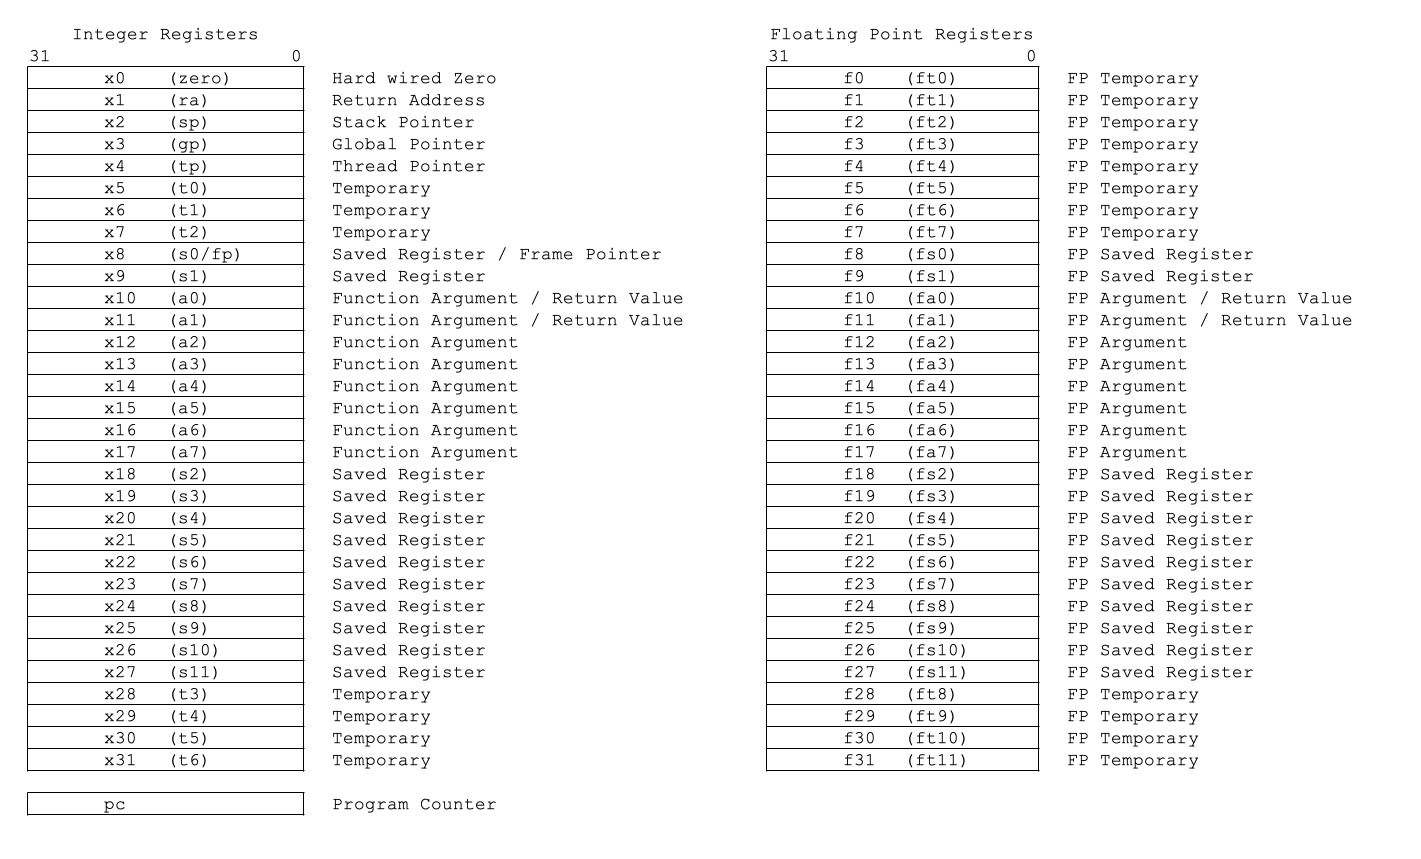
\includegraphics[width=0.9\columnwidth]{./Figure/ProgrammersModel_RV32IMAFC.png}
    \caption{Programmers Model for RV32IM[A][F][C]}
    \label{fig:PROGRAMMERSMODEL_RV32IMAFC}
\end{figure}

\begin{figure}[H]
    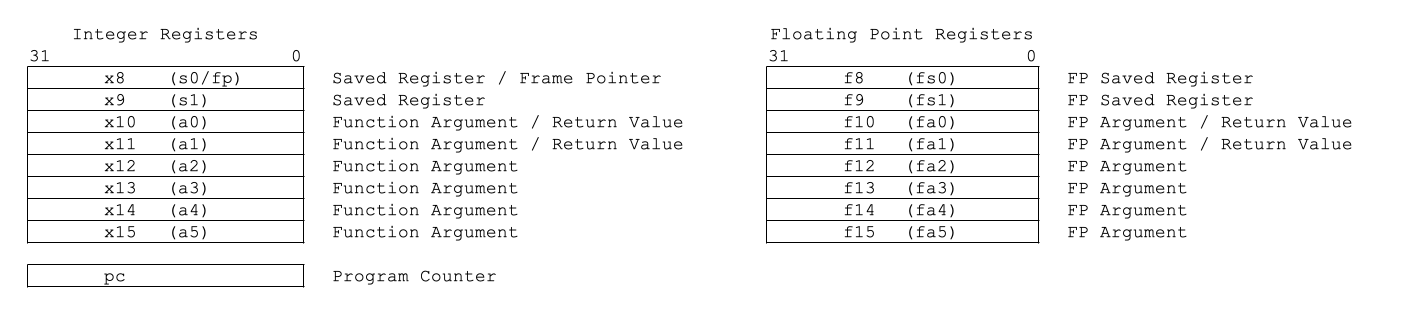
\includegraphics[width=0.9\columnwidth]{./Figure/ProgrammersModel_RV32CF.png}
    \caption{Programmers Model for RV32C/RV32CF\\(Compressed Instruction)}
    \label{fig:PROGRAMMERSMODEL_RV32CF}
\end{figure}

\begin{figure}[H]
    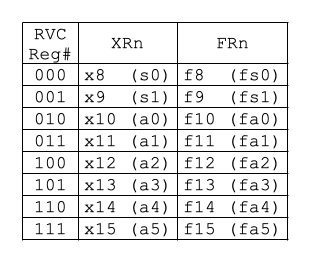
\includegraphics[width=0.2\columnwidth]{./Figure/ProgrammersModel_RV32CF_RegNum.png}
    \caption{Register Number Indication for RV32C/RV32CF\\(Compressed Instruction)}
    \label{fig:PROGRAMMERSMODEL_RV32CF_REGNUM}
\end{figure}

